\documentclass[12pt, notitlepage, final]{article} 

\newcommand{\name}{Vince Coghlan}

\usepackage{amsfonts}
\usepackage{amssymb}
\usepackage{amsmath}
\usepackage{latexsym}
\usepackage{enumerate}
\usepackage{amsthm}
\usepackage{nccmath}
\usepackage{setspace}
\usepackage[pdftex]{graphicx}
\usepackage{epstopdf}
\usepackage[siunitx]{circuitikz}
\usepackage{tikz}
\usepackage{float}
\usepackage{cancel}
\usepackage{pgfplots}
\usepackage{setspace}
\usepackage{overpic}
\usepackage{mathtools}
\usepackage{listings}
\usepackage{color}
\usepackage{hyperref}
\usepackage{gensymb}

\numberwithin{equation}{section}
\DeclareRobustCommand{\beginProtected}[1]{\begin{#1}}
\DeclareRobustCommand{\endProtected}[1]{\end{#1}}
\newcommand{\dbr}[1]{d_{\mbox{#1BR}}}
\newtheorem{lemma}{Lemma}
\newtheorem*{corollary}{Corollary}
\newtheorem{theorem}{Theorem}
\newtheorem{proposition}{Proposition}
\theoremstyle{definition}
\newtheorem{define}{Definition}
\newcommand{\column}[2]{
\left( \begin{array}{ccc}
#1 \\
#2
\end{array} \right)}

\newdimen\digitwidth
\settowidth\digitwidth{0}
\def~{\hspace{\digitwidth}}

\setlength{\parskip}{1pc}
\setlength{\parindent}{0pt}
\setlength{\topmargin}{-3pc}
\setlength{\textheight}{9.0in}
\setlength{\oddsidemargin}{0pc}
\setlength{\evensidemargin}{0pc}
\setlength{\textwidth}{6.5in}
\newcommand{\answer}[1]{\newpage\noindent\framebox{\vbox{{\bf ECEN 4797 Fall 2014}
\hfill {\bf \name} \vspace{-1cm}
\begin{center}{Homework \#5}\end{center} } }\bigskip }

%absolute value code
\DeclarePairedDelimiter\abs{\lvert}{\rvert}%
\DeclarePairedDelimiter\norm{\lVert}{\rVert}
\makeatletter
\let\oldabs\abs
\def\abs{\@ifstar{\oldabs}{\oldabs*}}
%
\let\oldnorm\norm
\def\norm{\@ifstar{\oldnorm}{\oldnorm*}}
\makeatother

\def\dbar{{\mathchar'26\mkern-12mu d}}
\def \Frac{\displaystyle\frac}
\def \Sum{\displaystyle\sum}
\def \Int{\displaystyle\int}
\def \Prod{\displaystyle\prod}
\def \P[x]{\Frac{\partial}{\partial x}}
\def \D[x]{\Frac{d}{dx}}
\newcommand{\PD}[2]{\frac{\partial#1}{\partial#2}}
\newcommand{\PF}[1]{\frac{\partial}{\partial#1}}
\newcommand{\DD}[2]{\frac{d#1}{d#2}}
\newcommand{\DF}[1]{\frac{d}{d#1}}
\newcommand{\fix}[2]{\left(#1\right)_#2}
\newcommand{\ket}[1]{|#1\rangle}
\newcommand{\bra}[1]{\langle#1|}
\newcommand{\braket}[2]{\langle #1 | #2 \rangle}
\newcommand{\bopk}[3]{\langle #1 | #2 | #3 \rangle}
\newcommand{\Choose}[2]{\displaystyle {#1 \choose #2}}
\newcommand{\proj}[1]{\ket{#1}\bra{#1}}
\def\del{\vec{\nabla}}
\newcommand{\avg}[1]{\langle#1\rangle}
\newcommand{\piecewise}[4]{\left\{\beginProtected{array}{rl}#1&:#2\\#3&:#4\endProtected{array}\right.}
\newcommand{\systeme}[2]{\left\{\beginProtected{array}{rl}#1\\#2\endProtected{array}\right.}
\def \KE{K\!E}
\def\Godel{G$\ddot{\mbox{o}}$del}

\onehalfspacing

\begin{document}

\answer{}

\textbf{5.1:} This problem uses information extracted from portions of the data sheet
for a Vishay Siliconix power MOSFET SiHF620 (the full datasheet is available at
\url{http://www.vishay.com/docs/91027/sihf620.pdf)}. The on- state resistance of this MOSFET
($R_\text{DS(on)}$) is $0.8\Omega$ at $25\degree$ C. This on-state resistance varies with junction
temperature, as illustrated in Fig. 4 (note that Fig.4 plots the normalized variation).
The junction-to-case thermal resistance ($R_\text{thJC}$) is $2.5\degree$ C/W (see above table).
Also the junction-to-case transient thermal impedance versus pulse duration, for a single
rectangular power dissipation pulse and repeated pulses of different duty ratios, is
given in Fig. 11. For both parts of this problem assume that the maximum allowable
junction temperature ($T_J$) is $140\degree$ C and the maximum ambient temperature ($T_A$)
is $50 \degree$ C.

\begin{enumerate}[(a)]
  \item{}The MOSFET is first attached to a heat sink using an insulating pad resulting
    in a case-to-sink thermal resistance ($R_\text{thCS}$) of $0.75\degree$ C/W. Assuming that the
    MOSFET must carry a (forward) rms current of 2.5 A, and that switching losses can be
    ignored, what is the maximum allowable thermal resistance of the heat sink ($R_{\text{thSA}}$)?\\

    We can use an equivalent circuit to aid in our understanding.  This would consist of the
    junction-to-case thermal resistance, the case-to-sink thermal resistance, and the thermal
    resistance of the sink itself, all in series.  Power lost will be the current times the voltage,
    or, at the maximum allowable junction temperature (note that the resistance has been denormalized),
    $2.5$ A $\cdot$ $(1.7\cdot2.5)$ V $=10.63$ W.
    This will act as the current into this system, the equation can thus be set up:
    \[
      T_J - T_A = P_{loss}(R_{th(JC)}+R_{th(CS)}+R_{th(SA)})
    \]
    \[
      90 = 10.63(2.5 + 0.75 + R_{th(SA)}) \Rightarrow R_{th(SA)} = 5.22 \degree C/W
    \]

  \item{}The MOSFET is now instead operated in a pulsed fashion, carrying rectangular pulses
    of current of magnitude $I_p$, 1 ms in duration with 99 ms of off time between pulses.
    If the MOSFET is mounted to an extremely good heat sink that maintains the case temperature
    at $50\degree$ C, what is the maximum allowable current pulse magnitude ($I_p$)? You may assume
    that the MOSFET on-state resistance is always at its $140\degree$ C value.

    The thermal response of the junction to the case is going to occur on the second to last line,
    that represents approximately a duty cycle of $\frac{1}{99}$.  At 0.001 seconds the approximate
    thermal response is 0.25 $\Omega$.  We know that:
    \[
      T_J = P Z_{Th(JC)} + T_C \Rightarrow 140 = I_p^2\cdot1.7\cdot0.25 + 50
    \]
    And thus:
    \[
      I_p = 14.55 A
    \]
\end{enumerate}

\textbf{5.2:} The elements of the buck-boost converter of Fig 5.21 are ideal: all losses may be
ignored.  Your results for parts (a) and (b) should agree with Table 5.2.

\begin{center}
      \begin{circuitikz}[american]
       \draw
       (0, 0) to [V=$V_g$] (0, 3)
       (1.5,3) node[nmos, rotate=90] (n) {}
       (0, 3) to[short] (1,3)
       (2,3) to[short] (3, 3)
       to [L=$L$,i=$i(t)$] (3, 0)
         to [short] (0,0)
       (5,3) to[D*=$D_1$,/tikz/circuitikz/bipoles/length=1cm] (3,3)
       (5,3) to [C=$C$] (5,0)
         to [short] (3,0)
       (5,3) to[short] (7,3)
         to [R=$R$,v=$V$] (7,0)
         to[short] (5,0)
     ;\end{circuitikz}
    \end{center}

\begin{enumerate}[(a)]
  \item{}Show that the converter operates in discontinuous conduction mode when $K<K_{crit}$, and
    derive expressions for $K$ and $K_{crit}$.\\
      We can use some previous techniques to find the values of the ripple voltage and the current.
      In state 1:
      \[
        i_C=-i_L-\frac{V}{R} \text{ and } V_L = V
      \]
      In two:
      \[
        i_C=\frac{-V}{R} \text{ and } V_L = V_g
      \]
      With this we can derive some PSS equations:
      \[
        0 = (-i_L-\frac{V}{R})D' + -\frac{V}{R}D
      \]
      \[
        0 = VD'+V_gD
      \]
      Which gives us some more equations:
      \[
        V=\frac{-V_gD}{D'} \text{ and } i_L=\frac{-V}{RD'}
      \]
      We know that $V_L=L\frac{di_L}{dt}$, and with that we can solve for the ripple current:
      \[
        \Delta i_L = \frac{V_g}{2L}
      \]
      We can also derive a more general equation for the average inductor current by plugging
      in for V:
      \[
        i_L = \frac{V_gD}{R{D'}^2}
      \]
      We can now generate our equality knowing that $I_L - \Delta i_LDT_s < 0$:
      \[
        \frac{V_gD}{R{D'}^2}-\frac{V_gDT_s}{2L} < 0 \Rightarrow \frac{2L}{T_sR} < {D'}^2
      \]
      Also known as $(1-D)^2$.  This shows us that $K=\frac{2L}{T_sR}$ and $K_{crit}=(1-D)^2$ and
      clearly when $K < K_{crit}$ we will have a negative current at some point.

  \item{}Derive an expression for the dc conversion ratio $V/V_g$ of the buck-boost converter
    operating in discontinuous conduction mode.\\
    Using our equation for the average voltage we know that:
    \[
      V=\frac{-V_gD_1}{D_2} \Rightarrow D_2 = \frac{-V_gD_1}{V}
    \]
    The we can find the current through our diode, assuming the average current is 0, we know:
    \[
      i_D = -<i_C> - \frac{V}{R} = \frac{-V}{R}
    \]
    We also know that the peak inductor current is going to go through the entire diode during
    the $D_2$ period, we can find this:
    \[
      i_D = \frac{1}{T_s}(T_sD_2i_{peak})
    \]
    A simple derivation of $i_{peak}$ can be seen below:
    \[
      V_g = L\frac{di}{dt} \Rightarrow \Delta i_L = \frac{V}{2L}
    \]
    \[
      i_{peak} = \Delta i_L\cdot D_1\cdot T_s \Rightarrow i_{peak} = \frac{V_g}{2L}D_1T_s
    \]
    This tells us:
    \[
      i_D = D_2\frac{V_g}{2L}D_1\cdot T_s
    \]
    Now setting these equal we find:
    \[
      \frac{-V}{R} = D_2\frac{V_g}{2L}D_1\cdot T_s \Rightarrow \frac{V}{V_g} = \frac{-D_2D_1T_sR}{2L}
    \]
    Plugging in $\frac{-V_gD_1}{V}$ for $D_2$ and substituting our $K$ from the last problem we get:
    \[
      (\frac{V}{V_g})^2 = \frac{{D_1}^2}{K} \Rightarrow \frac{V}{V_g} = \pm\frac{D_1}{\sqrt{K}}
    \]
    We know that this value will be negative since our output voltage must be negative, this means
    that our final conversion factor is: $\frac{-D_1}{\sqrt{K}}$.

  \item{}For $K=0.1$, plot $V/V_g$ over the entire range $0\leq D\leq1$.\\
    \begin{figure}[H]
    \begin{center}
    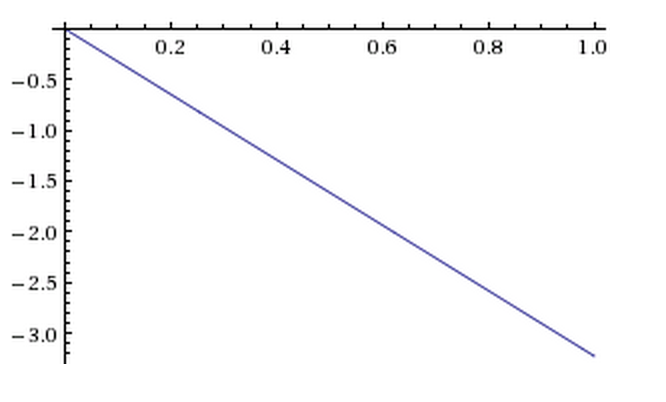
\includegraphics[width=7cm]{f1}
    \end{center}
    \end{figure}

  \item{}Sketch the inductor voltage and current waveforms for $K=1$ and $D=0.3$.  Label salient
    features.\\

    The inductor voltage will be $V_L = L$, (from lecture notes)

    \begin{figure}[H]
    \begin{center}
    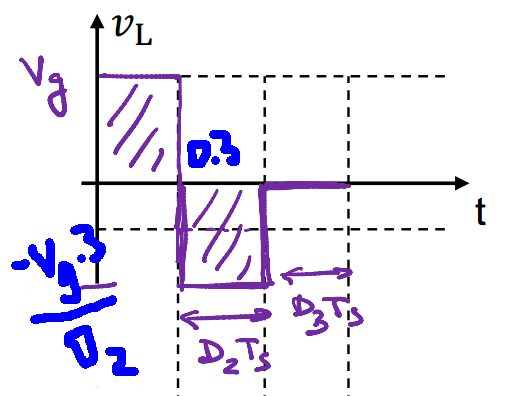
\includegraphics[width=7cm]{f2}
    \end{center}
    \end{figure}

    The current waveforms will look like (also from the lecture notes):

    \begin{figure}[H]
    \begin{center}
    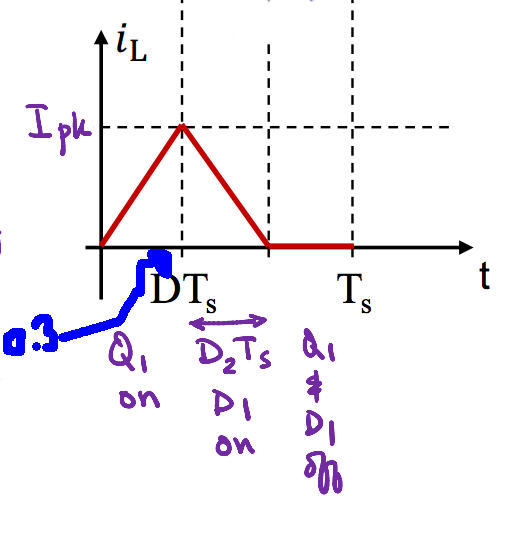
\includegraphics[width=7cm]{f3}
    \end{center}
    \end{figure}


  \item{}What happens to $V$ at no load $(R\rightarrow \infty)$? Explain why, physically.\\
    When there is no resistor, the voltage goes to negative infinity.  The reason is because
    every period we pull current from the diode, and the diode never lets us put any back.  Since
    we have just a capacitor, none of the voltage can escape, and it keeps building up.
    This can be seen in the equation found above.

\end{enumerate}


\end{document}
